% NVIDIA ATE Test Methodology Engineer - interview project presentation
% Standalone, editable 16:9 Beamer. No external assets required.
% Source projects: Software-Projects/main.tex and EDA-CAD-Project/main.tex.
% Scope: NeoPower scenario-based testing, earlier ABC SO/MO mapping research.
% Not an ATE silicon test experience claim. Rehearsal target: 10-12 minutes.
\documentclass[aspectratio=169,10pt]{beamer}
\usepackage[english]{babel}
\usepackage[utf8]{inputenc}
\usepackage[T1]{fontenc}
\usepackage{lmodern}
\usepackage{amsmath,amssymb}
\usepackage{graphicx}
\usepackage{xcolor}
\usepackage{tikz}
\usetikzlibrary{arrows.meta,positioning,calc,fit,backgrounds,shapes.geometric}
\usepackage{hyperref}
\hypersetup{hidelinks}

% Match the visual identity of the existing Software / EDA-CAD decks.
\usetheme{Madrid}
\usecolortheme{default}
\definecolor{Ink}{HTML}{243748}
\definecolor{Muted}{HTML}{667B8B}
\definecolor{Accent}{HTML}{347E74}
\definecolor{AccentBlue}{HTML}{507DAD}
\definecolor{SoftMint}{HTML}{E6F4EE}
\definecolor{SoftBlue}{HTML}{E9F2F9}
\definecolor{SoftLilac}{HTML}{F1EEF8}
\definecolor{Paper}{HTML}{FBFCFE}
\definecolor{Divider}{HTML}{D8E4EB}
\setbeamercolor{background canvas}{bg=Paper}
\setbeamercolor{normal text}{fg=Ink}
\setbeamercolor{structure}{fg=Accent}
\setbeamercolor{frametitle}{fg=Ink,bg=SoftBlue}
\setbeamercolor{title}{fg=Ink}
\setbeamercolor{subtitle}{fg=Muted}
\setbeamercolor{block title}{fg=Ink,bg=SoftBlue}
\setbeamercolor{block body}{fg=Ink,bg=white}
\setbeamercolor{item}{fg=Accent}
\setbeamercolor{footline}{fg=Muted,bg=Paper}
\setbeamercolor{panelblue}{fg=Ink,bg=SoftBlue!70}
\setbeamercolor{panelmint}{fg=Ink,bg=SoftMint!80}
\setbeamercolor{panellilac}{fg=Ink,bg=SoftLilac!90}
\setbeamercolor{panelwhite}{fg=Ink,bg=white}
\setbeamerfont{frametitle}{size=\Large,series=\bfseries}
\setbeamerfont{footline}{size=\tiny}
\setbeamertemplate{headline}{}
\setbeamertemplate{navigation symbols}{}
\setbeamertemplate{blocks}[rounded][shadow=false]
\setbeamertemplate{itemize items}[circle]
\setbeamertemplate{footline}{%
  \leavevmode\hbox{%
    \begin{beamercolorbox}[wd=\paperwidth,ht=.30cm,dp=.16cm,rightskip=.60cm plus 1fil]{footline}%
      \hfill\insertframenumber\,/\,\inserttotalframenumber
    \end{beamercolorbox}}%
}
\setbeamertemplate{frametitle}{%
  \nointerlineskip
  \begin{beamercolorbox}[wd=\paperwidth,ht=.77cm,dp=.18cm,leftskip=.64cm]{frametitle}%
    \usebeamerfont{frametitle}\insertframetitle
  \end{beamercolorbox}%
}
\newcommand{\smalllabel}[1]{{\scriptsize\bfseries\color{Accent}\MakeUppercase{#1}}}
\newcommand{\takeaway}[1]{%
  \begin{beamercolorbox}[rounded=true,sep=0.13cm,wd=\linewidth]{block title}%
    \raggedright\strut\textbf{#1}\strut
  \end{beamercolorbox}%
}
\newcommand{\softpanel}[3]{%
  \begin{beamercolorbox}[rounded=true,sep=0.16cm,wd=\linewidth]{#1}%
  {\small\bfseries\color{Accent}#2}\par\vspace{0.06cm}
  {\small\color{Ink}#3}
  \end{beamercolorbox}%
}
\tikzset{
  flow/.style={draw=AccentBlue!70,fill=SoftBlue,rounded corners=3pt,
    line width=0.8pt,align=center,text width=2.45cm,minimum height=1.0cm,
    inner sep=4pt,font=\small},
  mint/.style={flow,draw=Accent!75,fill=SoftMint},
  lilac/.style={flow,draw=AccentBlue!45,fill=SoftLilac},
  outline/.style={flow,draw=Divider,fill=white},
  wideflow/.style={flow,text width=3.25cm,minimum height=1.15cm},
  mini/.style={draw=Divider,fill=white,rounded corners=3pt,
    align=center,text width=2.55cm,minimum height=.80cm,
    inner sep=3pt,font=\small},
  arr/.style={-Latex,thick,draw=Accent},
  arrblue/.style={-Latex,thick,draw=AccentBlue},
}
\title{Software Engineering \& Test Methodology}
\subtitle{Scenario-Based Simulation / C++ Algorithms / Verification}
\author{Yu-Jui (Stanley) Liang}
\institute{National Taiwan University}
\date{November 2026}
\begin{document}

% 01 / COVER -----------------------------------------------------
{\setbeamertemplate{footline}{}
\begin{frame}[plain]
  \vspace*{.88cm}
  {\normalsize\bfseries\color{Accent}NVIDIA ATE TEST METHODOLOGY ENGINEER}\par
  \vspace{.44cm}
  {\fontsize{23}{27}\selectfont\bfseries\color{Ink}Software Engineering\\[2mm]\& Test Methodology}\par
  \vspace{.28cm}
  {\color{Muted}\fontsize{11}{14}\selectfont
     Scenario-Based Simulation\quad $\cdot$\quad C++ Algorithm Development\quad $\cdot$\quad Verification}\par
  \vspace{.70cm}
  {\large\bfseries Yu-Jui (Stanley) Liang}\par
  {\small\color{Muted}National Taiwan University}\par
  \vfill
\end{frame}}

% 02 / BACKGROUND -----------------------------------------------
\begin{frame}{Education \& Engineering Background}
  \vspace{.07cm}
  \begin{columns}[T,onlytextwidth]
  \begin{column}{.49\textwidth}
    \begin{beamercolorbox}[rounded=true,sep=.21cm,wd=\linewidth]{panelblue}
      {\large\bfseries\color{AccentBlue}Education}\par\vspace{.22cm}
      {\normalsize\bfseries National Taiwan University}\par\vspace{.05cm}
      {\normalsize M.S. Candidate, Data Science}\par
      {\small\color{Muted}Expected graduation: Jul.--Sep. 2027}\par
      \vspace{.35cm}{\color{Divider}\rule{.96\linewidth}{.5pt}}\par\vspace{.22cm}
      {\normalsize\bfseries National Chengchi University}\par\vspace{.05cm}
      {\normalsize B.S. in Computer Science}\par
      {\normalsize Double Major in Electro-Physics}\par
      {\small\color{Muted}Sep. 2021 -- Jun. 2025}\par
    \end{beamercolorbox}
  \end{column}
  \begin{column}{.49\textwidth}
    \begin{beamercolorbox}[rounded=true,sep=.21cm,wd=\linewidth]{panelmint}
      {\large\bfseries\color{Accent}Engineering Experience}\par\vspace{.22cm}
      {\normalsize\bfseries NeoPower Technologies}\par\vspace{.05cm}
      {\normalsize Contract Software Engineer}\par
      {\small\color{Muted}Backend development / simulator / debugging}\par
      \vspace{.34cm}{\color{Divider}\rule{.96\linewidth}{.5pt}}\par\vspace{.22cm}
      {\normalsize\bfseries AIMobile (Inventec Group)}\par\vspace{.05cm}
      {\normalsize Contract Software Engineer}\par
      {\small\color{Muted}Software modules / integration / validation}\par
    \end{beamercolorbox}
  \end{column}
  \end{columns}
  \vspace{.26cm}
  \takeaway{Focus: testing, tools, and verification.}
\end{frame}

% 03 / SYSTEM ARCHITECTURE --------------------------------------
\begin{frame}{NeoPower: Backend System Architecture}
  \takeaway{Electric-bus charging management platform with multiple external vendors.}
  \vspace{.24cm}
  \centering
  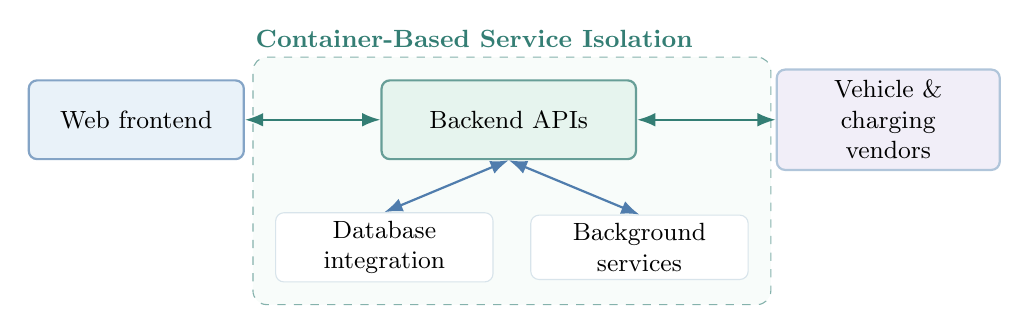
\begin{tikzpicture}[>=Latex]
    \node[flow] (ui) at (0,0) {Web frontend};
    \node[mint,text width=2.95cm] (api) at (4.73,0) {Backend APIs};
    \node[lilac,text width=2.55cm] (vendor) at (9.55,0) {Vehicle \& charging\\vendors};
    \node[mini] (db) at (3.15,-1.62) {Database\\integration};
    \node[mini] (jobs) at (6.39,-1.62) {Background\\services};
    \begin{scope}[on background layer]
       \node[draw=Accent!60,dashed,fill=SoftMint!28,rounded corners=5pt,
       inner xsep=8pt,inner ysep=8pt,fit={(api)(db)(jobs)}] (boundary) {};
    \end{scope}
    \node[anchor=south west,font=\small\bfseries,text=Accent,inner sep=1pt]
      at ([yshift=2pt]boundary.north west) {Container-Based Service Isolation};
    \draw[<->,Accent,thick] (ui) -- (api);
    \draw[<->,Accent,thick] (api) -- (vendor);
    \draw[<->,AccentBlue,thick] (api.south) -- (db.north);
    \draw[<->,AccentBlue,thick] (api.south) -- (jobs.north);
  \end{tikzpicture}
  \par\vspace{.22cm}
  {\small\bfseries\color{Accent}My contributions}\par\vspace{.07cm}
  {\small Backend APIs and database integration\quad /\quad Log analysis and debugging\par
    \vspace{.05cm}Software integration\quad /\quad Deployment and maintenance}
\end{frame}

% 04 / SIMULATOR -----------------------------------------------
\begin{frame}{NeoPower: Scenario-Based System Simulation}
  \takeaway{I developed a custom simulator to reproduce vendor interactions and failures.}
  \vspace{.20cm}
  \centering
  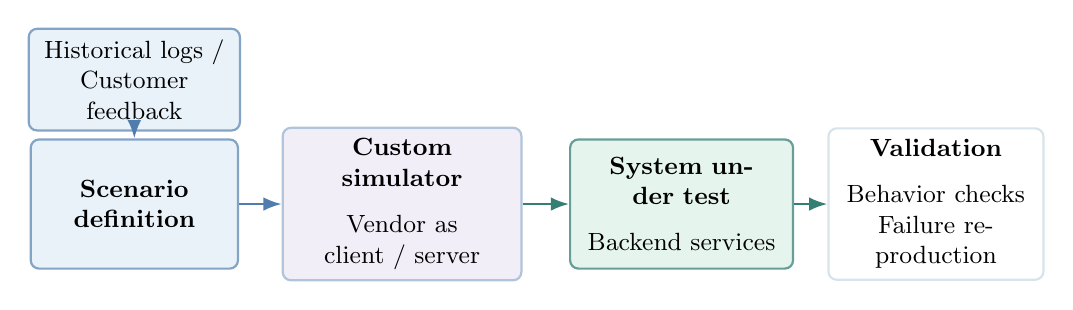
\begin{tikzpicture}[>=Latex]
    \node[flow,text width=2.40cm,minimum height=.75cm] (logs) at (0,1.46)
       {Historical logs /\\Customer feedback};
    \node[flow,text width=2.35cm,minimum height=1.64cm] (scenario) at (0,-.12)
       {\textbf{Scenario}\\\textbf{definition}};
    \node[lilac,text width=2.75cm,minimum height=1.64cm] (sim) at (3.40,-.12)
       {\textbf{Custom simulator}\\[2mm]Vendor as\\client / server};
    \node[mint,text width=2.55cm,minimum height=1.64cm] (sut) at (6.95,-.12)
       {\textbf{System under test}\\[2mm]Backend services};
    \node[outline,text width=2.45cm,minimum height=1.64cm] (result) at (10.18,-.12)
       {\textbf{Validation}\\[2mm]Behavior checks\\Failure reproduction};
    \draw[arrblue] (logs) -- (scenario);
    \draw[arrblue] (scenario) -- (sim);
    \draw[arr] (sim) -- (sut);
    \draw[arr] (sut) -- (result);
  \end{tikzpicture}
  \par\vspace{.25cm}
  \begin{columns}[T,onlytextwidth]
    \begin{column}{.49\textwidth}
       \softpanel{panelblue}{High-Load Scenario}{Many buses arrive together; charging requests increase.}
    \end{column}
    \begin{column}{.49\textwidth}
       \softpanel{panelmint}{Network-Failure Scenario}{Multiple chargers or stations disconnect at the same time.}
    \end{column}
  \end{columns}
\end{frame}

% 05 / TESTING + VALIDATION ------------------------------------
\begin{frame}{NeoPower: Testing \& Production Reliability}
  \begin{columns}[T,onlytextwidth]
    \begin{column}{.44\textwidth}
      {\normalsize\bfseries\color{AccentBlue}Pre-Deployment Testing}\par\vspace{.22cm}
      \centering
      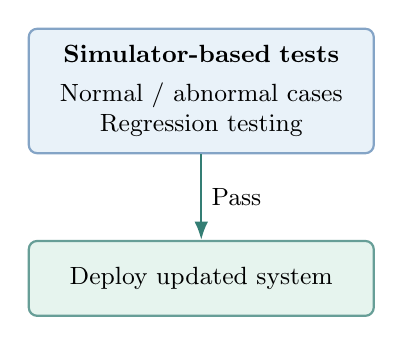
\begin{tikzpicture}[>=Latex]
        \node[flow,text width=4.1cm,minimum height=1.58cm] (test) at (0,0)
           {\textbf{Simulator-based tests}\\[1mm]Normal / abnormal cases\\Regression testing};
        \node[mint,text width=4.1cm,minimum height=.95cm] (deploy) at (0,-2.38)
           {Deploy updated system};
        \draw[arr] (test) -- node[right,font=\small] {Pass} (deploy);
      \end{tikzpicture}
    \end{column}
    \begin{column}{.54\textwidth}
      {\normalsize\bfseries\color{Accent}Post-Deployment Validation}\par\vspace{.22cm}
      {\small Charging-power allocation algorithms}\par\vspace{.17cm}
      \centering
      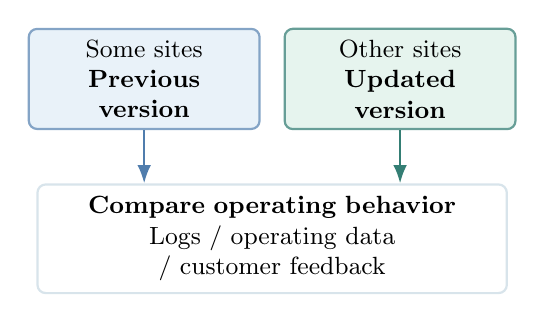
\begin{tikzpicture}[>=Latex]
        \node[flow,text width=2.65cm,minimum height=1.10cm] (old) at (0,0)
          {Some sites\\\textbf{Previous version}};
        \node[mint,text width=2.65cm,minimum height=1.10cm] (new) at (3.25,0)
          {Other sites\\\textbf{Updated version}};
        \node[outline,text width=5.68cm,minimum height=1.38cm] (eval) at (1.625,-2.03)
          {\textbf{Compare operating behavior}\\Logs / operating data / customer feedback};
        \draw[arrblue] (old.south) -- (old.south |- eval.north);
        \draw[arr] (new.south) -- (new.south |- eval.north);
      \end{tikzpicture}
    \end{column}
  \end{columns}
  \vspace{.29cm}
  \takeaway{Testing is repeatable before release; operational data supports follow-up evaluation.}
\end{frame}

% 06 / MAPPING MOTIVATION --------------------------------------
\begin{frame}{Earlier Research: Why Multi-Output Mapping?}
  \takeaway{Standard-cell mapping can jointly implement correlated output functions.}
  \vspace{.22cm}
  \centering
  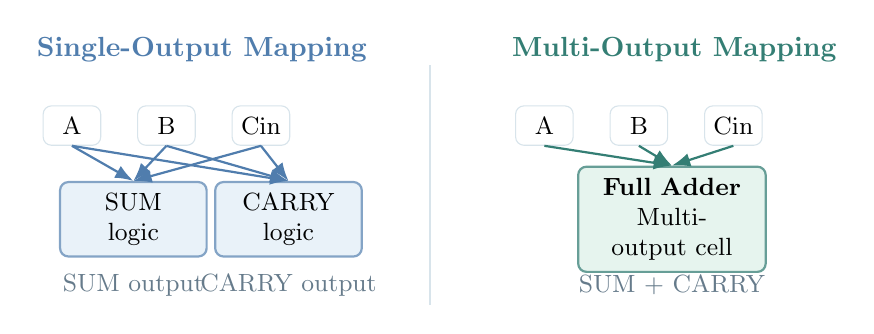
\begin{tikzpicture}[>=Latex]
    \node[font=\normalsize\bfseries,text=AccentBlue] at (2.65,2.0) {Single-Output Mapping};
    \node[font=\normalsize\bfseries,text=Accent] at (8.65,2.0) {Multi-Output Mapping};
    % left AIG/individual implementation
    \foreach \x/\lab in {1.0/A,2.2/B,3.4/Cin} {
      \node[mini,text width=.52cm,minimum height=.50cm] (l\lab) at (\x,1.03) {\lab};
      \node[mini,text width=.52cm,minimum height=.50cm] (r\lab) at (\x+6.0,1.03) {\lab};
    }
    \node[flow,text width=1.58cm,minimum height=.82cm] (s) at (1.78,-.16) {SUM\\logic};
    \node[flow,text width=1.58cm,minimum height=.82cm] (c) at (3.75,-.16) {CARRY\\logic};
    \node[mint,text width=2.10cm,minimum height=1.08cm] (fa) at (8.62,-.16) {\textbf{Full Adder}\\Multi-output cell};
    \foreach \n in {lA,lB,lCin} {
      \draw[arrblue] (\n.south) -- (s.north);
      \draw[arrblue] (\n.south) -- (c.north);
    }
    \foreach \n in {rA,rB,rCin} {\draw[arr] (\n.south) -- (fa.north);}
    \node[font=\small,text=Muted] at (1.78,-1.0) {SUM output};
    \node[font=\small,text=Muted] at (3.75,-1.0) {CARRY output};
    \node[font=\small,text=Muted] at (8.62,-1.0) {SUM + CARRY};
    \draw[Divider,thick] (5.55,-1.25) -- (5.55,1.80);
  \end{tikzpicture}
  \par\vspace{.19cm}
  {\small\color{Muted}One full-adder cell may replace multiple single-output cells when both outputs share a valid input and pin mapping.}
\end{frame}

% 07 / END-TO-END PIPELINE --------------------------------------
\begin{frame}{C++ EDA Project: Joint SO/MO Mapping Pipeline}
  \takeaway{Extend ABC's mapping path while preserving single-output alternatives.}
  \vspace{.33cm}
  \centering
  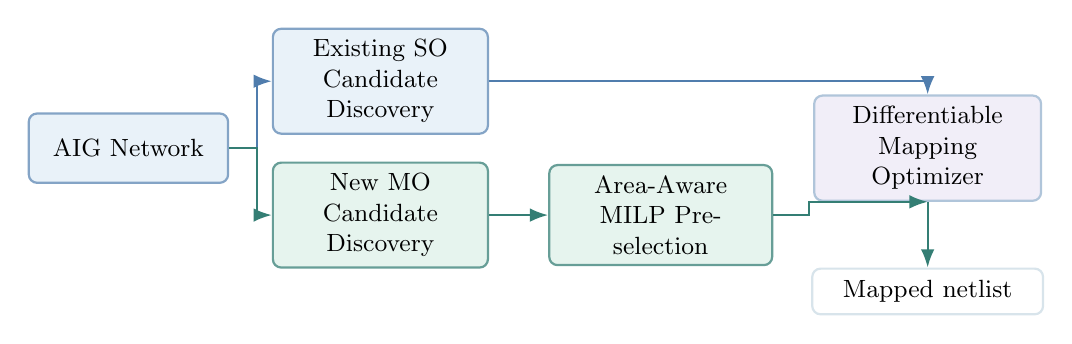
\begin{tikzpicture}[>=Latex]
    \node[flow,text width=2.25cm,minimum height=.88cm] (aig) at (0,1.15) {AIG Network};
    \node[flow,text width=2.45cm,minimum height=1.03cm] (so) at (3.20,2.00)
       {Existing SO\\Candidate Discovery};
    \node[mint,text width=2.45cm,minimum height=1.03cm] (mo) at (3.20,.30)
       {New MO\\Candidate Discovery};
    \node[mint,text width=2.55cm,minimum height=1.08cm] (milp) at (6.76,.30)
       {Area-Aware\\MILP Preselection};
    \node[lilac,text width=2.60cm,minimum height=1.20cm] (opt) at (10.15,1.15)
       {Differentiable\\Mapping Optimizer};
    \draw[arrblue] (aig.east) -- ++(.35,0) |- (so.west);
    \draw[arr] (aig.east) -- ++(.35,0) |- (mo.west);
    \draw[arr] (mo) -- (milp);
    \draw[arrblue] (so.east) -- ++(1.20,0) -| (opt.north);
    \draw[arr] (milp.east) -- ++(.45,0) |- (opt.south);
    \node[outline,text width=2.65cm,minimum height=.58cm] (net) at (10.15,-.67)
       {Mapped netlist};
    \draw[arr] (opt) -- (net);
  \end{tikzpicture}
  \par\vspace{.12cm}
  \begin{columns}[T,onlytextwidth]
    \begin{column}{.49\textwidth}
      \softpanel{panelblue}{Existing Baseline}{SO candidates remain available throughout final mapping.}
    \end{column}
    \begin{column}{.49\textwidth}
      \softpanel{panelmint}{My Main Extension}{MO matching, conflict-aware selection, and integration.}
    \end{column}
  \end{columns}
\end{frame}

% 08 / CANDIDATE DISCOVERY --------------------------------------
\begin{frame}{Multi-Output Candidate Discovery}
  \takeaway{Both outputs must pass one joint Boolean and pin mapping check.}
  \vspace{.24cm}
  \centering
  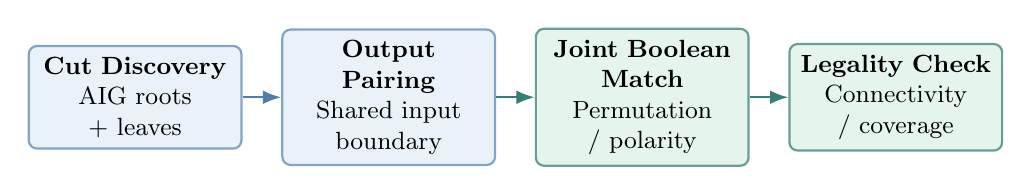
\begin{tikzpicture}[>=Latex]
    \node[flow,text width=2.42cm,minimum height=1.25cm] (cut) at (0,0)
       {\textbf{Cut Discovery}\\AIG roots + leaves};
    \node[flow,text width=2.42cm,minimum height=1.25cm] (pair) at (3.22,0)
       {\textbf{Output Pairing}\\Shared input boundary};
    \node[mint,text width=2.42cm,minimum height=1.25cm] (match) at (6.44,0)
       {\textbf{Joint Boolean Match}\\Permutation / polarity};
    \node[mint,text width=2.42cm,minimum height=1.25cm] (legal) at (9.66,0)
       {\textbf{Legality Check}\\Connectivity / coverage};
    \draw[arrblue] (cut) -- (pair);
    \draw[arr] (pair) -- (match);
    \draw[arr] (match) -- (legal);
  \end{tikzpicture}
  \par\vspace{.35cm}
  \begin{columns}[T,onlytextwidth]
  \begin{column}{.49\textwidth}
    \softpanel{panelblue}{Example: Full Adder}{SUM and CARRY may share cuts with leaves $\{A,B,C_{in}\}$.}
  \end{column}
  \begin{column}{.49\textwidth}
    \softpanel{panelmint}{Important Constraint}{Independent SO matches do not guarantee a legal common FA cell.}
  \end{column}
  \end{columns}
  \vspace{.28cm}
  {\small\color{Muted}Candidate matches are checked for functional equivalence and safe replacement connectivity.}
\end{frame}

% 09 / AREA AWARE MILP -----------------------------------------
\begin{frame}{Area-Aware Selection: MILP vs. FIFO}
  \takeaway{Select promising multi-output candidates without conflicting bindings.}
  \vspace{.18cm}
  \begin{columns}[T,onlytextwidth]
  \begin{column}{.51\textwidth}
    {\small\bfseries\color{AccentBlue}Overlapping output bindings}\par\vspace{.12cm}
    \centering
    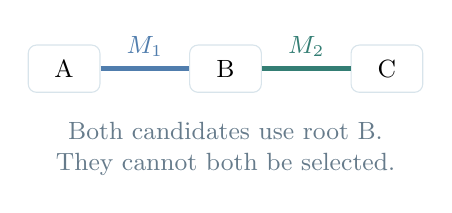
\begin{tikzpicture}[>=Latex]
      \node[mini,text width=.70cm,minimum height=.60cm] (a) at (0,0) {A};
      \node[mini,text width=.70cm,minimum height=.60cm] (b) at (2.05,0) {B};
      \node[mini,text width=.70cm,minimum height=.60cm] (c) at (4.10,0) {C};
      \draw[line width=2.0pt,AccentBlue] (a.east) -- node[above,font=\small,text=AccentBlue] {$M_1$} (b.west);
      \draw[line width=2.0pt,Accent] (b.east) -- node[above,font=\small,text=Accent] {$M_2$} (c.west);
      \node[font=\small,text=Muted,align=center] at (2.05,-1.02)
         {Both candidates use root B.\\They cannot both be selected.};
    \end{tikzpicture}
    \vspace{.18cm}
    \softpanel{panelblue}{FIFO Baseline}{Keep the first legal candidate; reject later conflicts.}
  \end{column}
  \begin{column}{.47\textwidth}
    {\small\bfseries\color{Accent}Optimization Model}\par\vspace{.10cm}
    {\scriptsize Binary variable $x_i \in\{0,1\}$ for each candidate.}\par\vspace{.20cm}
    \[
       \max \sum_i \Delta A_i x_i
    \]
    \vspace{-.26cm}
    {\scriptsize $\Delta A_i$: estimated SO area minus MO area.}\par\vspace{.07cm}
    \[
       \sum_{i:\,r\in C_i} x_i \leq 1
    \]
    \vspace{-.22cm}
    
  \end{column}
  \end{columns}
  \vspace{.05cm}
  {\small\color{Muted}MILP preselects candidates; the optimizer makes final mapping decisions.}
\end{frame}

% 10 / QUANTITATIVE RESULTS ------------------------------------
\begin{frame}{Normalized ADP Results}
  \takeaway{Area--Delay Product (ADP): lower is better.}
  \vspace{.22cm}
  \begin{columns}[T,onlytextwidth]
  \begin{column}{.62\textwidth}
    {\small\bfseries\color{AccentBlue}Geometric Mean of Normalized ADP}\par\vspace{.20cm}
    \centering
    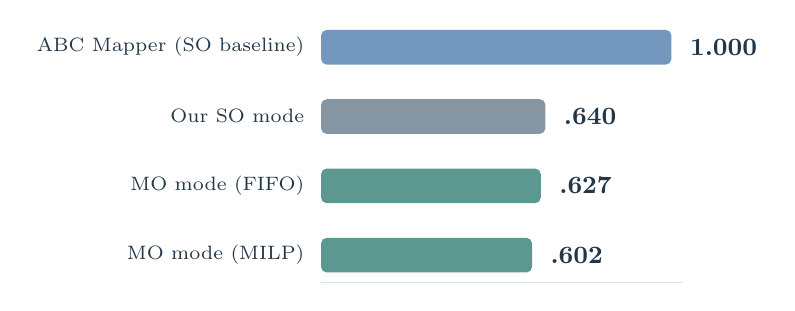
\begin{tikzpicture}[x=4.45cm,y=.88cm]
      \foreach \y/\label/\val/\col in {
        3/{ABC Mapper (SO baseline)}/1.000/AccentBlue,
        2/{Our SO mode}/.640/Muted,
        1/{MO mode (FIFO)}/.627/Accent,
        0/{MO mode (MILP)}/.602/Accent}
      {
        \node[anchor=east,font=\scriptsize,text=Ink] at (-.02,\y+.26) {\label};
        \fill[\col!80,rounded corners=2pt] (0,\y) rectangle (\val,\y+.50);
        \node[anchor=west,font=\small\bfseries,text=Ink] at (\val+.025,\y+.25) {\val};
      }
      \draw[draw=Divider] (0,-.14) -- (1.03,-.14);
    \end{tikzpicture}
  \end{column}
  \begin{column}{.36\textwidth}
    \begin{beamercolorbox}[rounded=true,sep=.15cm,wd=\linewidth]{panelmint}
      {\fontsize{22}{25}\selectfont\bfseries\color{Accent}6\%}\par\vspace{.07cm}
      {\small\bfseries Lower ADP vs. our SO mode}\par
      {\scriptsize\color{Muted}MILP MO: 0.602 vs. SO: 0.640}
    \end{beamercolorbox}
    \vspace{.18cm}
    \begin{beamercolorbox}[rounded=true,sep=.15cm,wd=\linewidth]{panelblue}
      {\fontsize{19}{22}\selectfont\bfseries\color{AccentBlue}4\%}\par\vspace{.07cm}
      {\small\bfseries Lower ADP vs. FIFO MO}\par
      {\scriptsize\color{Muted}MILP MO: 0.602 vs. FIFO: 0.627}
    \end{beamercolorbox}
  \end{column}
  \end{columns}
  \vspace{.09cm}
  {\small\color{Muted}30 arithmetic-logic benchmarks; ASAP7 7nm standard-cell library.}
\end{frame}

% 11 / RELIABILITY ---------------------------------------------
\begin{frame}{Correctness, Regression \& Scalability}
  \takeaway{Algorithm improvements matter only if the mapping remains correct and practical.}
  \vspace{.24cm}
  \begin{columns}[T,onlytextwidth]
  \begin{column}{.49\textwidth}
     {\large\bfseries\color{AccentBlue}Correctness}\par\vspace{.18cm}
     \softpanel{panelblue}{SO Mapping Regression}{Check that existing SO candidate behavior remains unchanged after MO integration.}
     \vspace{.16cm}
     \softpanel{panelblue}{Combinational Equivalence Check}{Compare original Boolean logic with the mapped gate-level netlist.}
  \end{column}
  \begin{column}{.49\textwidth}
     {\large\bfseries\color{Accent}Scalability}\par\vspace{.18cm}
     \softpanel{panelmint}{Bounded Search}{Limit cuts to $K=3$ leaves; retain up to 128 MO matches per node.}
     \vspace{.16cm}
     \softpanel{panelmint}{Pruning \& Measurement}{Deduplicate candidates; monitor runtime and peak memory use.}
  \end{column}
  \end{columns}
  \vspace{.10cm}
  \begin{beamercolorbox}[rounded=true,sep=.12cm,wd=\linewidth]{panellilac}
    {\small\bfseries\color{Ink}Engineering principle:} {\small Verify functionality, regression coverage, and resource limits alongside QoR.}
  \end{beamercolorbox}
\end{frame}

% 12 / CONCLUSION ----------------------------------------------
{\setbeamertemplate{footline}{}
\begin{frame}[plain]
  \vspace*{.72cm}
  {\fontsize{23}{28}\selectfont\bfseries\color{Ink}Engineering Takeaways}\par
  \vspace{.44cm}
  \begin{columns}[T,onlytextwidth]
  \begin{column}{.49\textwidth}
    \softpanel{panelblue}{Scenario-Based Testing}{Build repeatable simulations to reproduce failures and support regression testing.}
  \end{column}
  \begin{column}{.49\textwidth}
    \softpanel{panelmint}{C++ Tool Development}{Extend complex algorithms while verifying correctness, performance, and maintainability.}
  \end{column}
  \end{columns}
  \vspace{.40cm}
  {\normalsize\color{Muted}I hope to apply these software and verification skills to robust semiconductor test methodology.}\par
  \vfill
  {\large\bfseries\color{Accent}Thank you. Questions \& Discussion}\par\vspace{.20cm}
\end{frame}}

\end{document}